\section{Diagramme de classes}
    \label{sec:diagClass}
    
    Le diagramme de classe détaillé dans cette section permet de mieux comprendre l'architecture interne de Glasir.
    
    \subsection{Classe centrale}
    	\label{sec:diagClassCentral}
    	La classe centrale du diagramme est \emph{BigGlasir}, illustrée sur la {\sc Figure}~\ref{fig:bigglasir}. C'est autour d'elle que s'articule l'ensemble des fonctionnalités de Glasir. \emph{BigGlasir} dispose de méthodes permettant de charger un ADTree depuis la bibliothèque de modèles, de lancer des instances d'ADTool afin d'afficher un ADTree, mais également de créer ou de charger un projet. Cette classe possède également des modules, décrit dans la {\sc Section}~{\ref{sec:diagClassMod}}, une bibliothèque de modèles, décrite dans la {\sc Section}~{\ref{sec:diagClassBib}}, et une liste des instances d'ADTool, décrite dans la {\sc section}~{\ref{sec:diagClassADT}}.
    	
    	\begin{figure}[H]
	        \centering
	        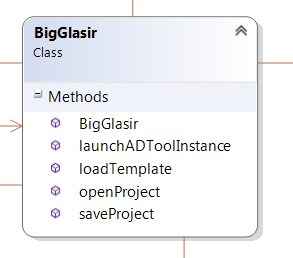
\includegraphics[height=0.3\textwidth]{figure/bigglasir.png}
	        \caption{Classe centrale gérant l'ensemble des autres fonctionnalités.}
	        \label{fig:bigglasir}
	    \end{figure}
    	
    \subsection{Instances d'ADTool}
    	\label{sec:diagClassADT}
    	
    	Comme mentionné dans le rapport de spécification, Glasir gère plusieurs instances d'ADTool pour permettre à l'utilisateur de travailler sur différents ADTrees en même temps\footnote{Pour rappel, ADTool ne peut gérer qu'un seul ADTree à la fois, il n'est par exemple pas possible d'ouvrir deux ADTrees en même temps pour les comparer.}. La classe \emph{ADToolInstance} contient donc le processus d'une instance d'ADTool, ainsi que le fichier de l'ADTree sur lequel l'instance porte. Ce fichier est représenté par la classe \emph{XMLFile}, qui contient un attribut pour représenter le nom du fichier, et des méthodes permettant d'opérer sur ce fichier, comme illustré sur la {\sc Figure}~\ref{fig:instADT}.
    	
    	
    	\begin{figure}[H]
	        \centering
	        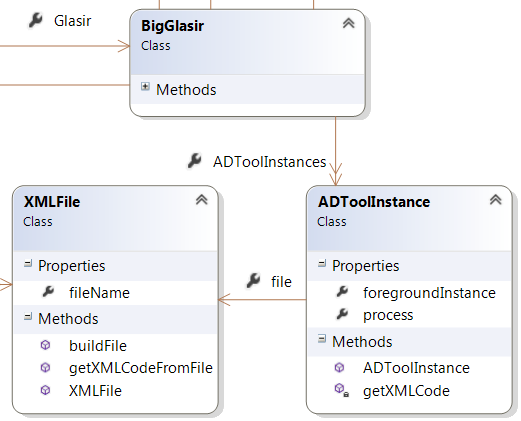
\includegraphics[height=0.5\textwidth]{figure/adtoolinstance.png}
	        \caption{Diagramme de classe des instances d'ADTool.}
	        \label{fig:instADT}
	    \end{figure}
	    


	\subsection{Modules}
    	\label{sec:diagClassMod}    	
    	
    	 Les trois modules principaux de Glasir, c'est-à-dire le Filtre, l'Optimiseur et l'Éditeur de fonction, ont chacun leur propre classe \emph{Filter}, \emph{Optimizer} et \emph{FunctionEditor}. Ces trois classes héritent de {\emph Module}, une classe abstaite contenant les méthodes communes aux trois modules, comme par exemple la méthode permettant d'ouvrir un fichier décrivant un ADTree. De plus, \emph{Module} contient des méthodes abstraites devant être implémentées dans chaque classe héritière, comme la méthode permettant par exemple d'obtenir le fichier résultant d'une opération appliquée par le module. La {\sc Figure}~\ref{fig:mod} illustre l'agencement de ces classes.
    	
    	
    	\begin{figure}[H]
	        \centering
	        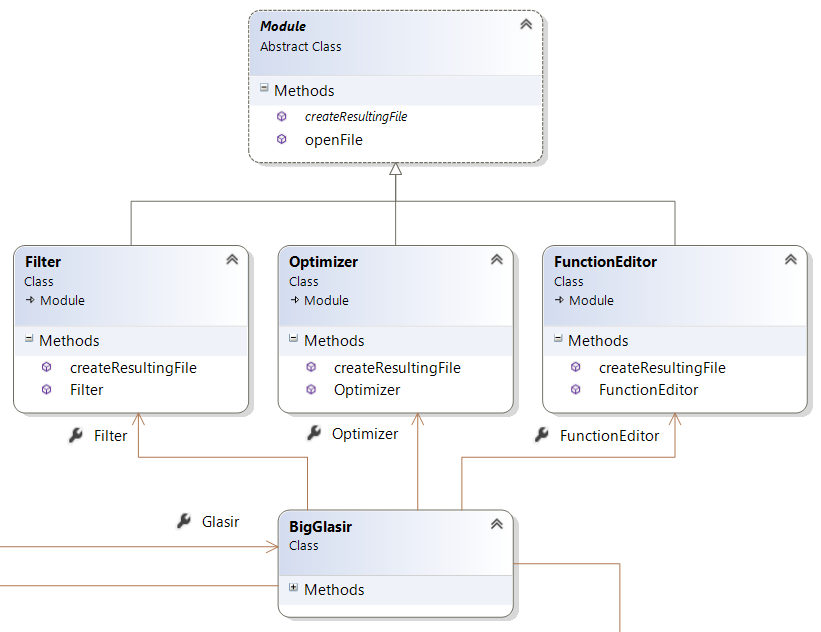
\includegraphics[height=0.7\textwidth]{figure/modules.png}
	        \caption{Diagramme de classe des trois modules de Glasir.}
	        \label{fig:mod}
	    \end{figure}
	    
	    
	\subsection{Bibliothèque de modèles}
    	\label{sec:diagClassBib}
    	La bibliothèque de modèle est constitué de la classe \emph{TemplateLibrary} qui contient une liste des fichiers modèles. Des méthodes permettent d'ajouter ou supprimer un ADTree de la bibliothèque, ou encore de charger un ADTree dans le projet courant. Les fichiers de cette bibliothèque sont là-aussi représentés par la classe \emph{XMLFile}, comme illustré sur la {\sc Figure}~\ref{fig:lib}.
    	
    	\begin{figure}[H]
	        \centering
	        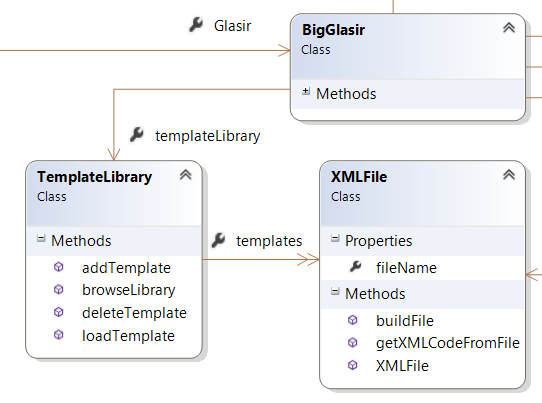
\includegraphics[height=0.5\textwidth]{figure/library.png}
	        \caption{Diagramme de classe de la bibliothèque de modèles.}
	        \label{fig:lib}
	    \end{figure}